\documentclass[11pt,a4paper]{article}
\usepackage[english]{babel}
\usepackage[nottoc]{tocbibind}

\usepackage{pgfplots}
\pgfplotsset{compat=1.18}

% \usepackage{geometry}
% \geometry{margin=1in}
% =========================
% Packages
% =========================
\usepackage[margin=1in]{geometry}
\usepackage{amsmath, amssymb, amsthm}
\usepackage{mathtools}
\usepackage{physics}
\usepackage{bm}
\usepackage{mathrsfs}

\usepackage{enumitem}
\usepackage{hyperref}
\usepackage{xcolor}
\usepackage{fancyhdr}
\usepackage{setspace}
\usepackage{graphicx}
\usepackage{xfrac}


\usepackage{forest}
\usepackage{tikz-qtree}
\usepackage{tikz}
\usetikzlibrary{arrows.meta}
% =========================
% Page Style
% =========================
\pagestyle{fancy}
\fancyhf{}
\lhead{\textsc{Lecture Notes}}
\rhead{\textsc{MAT211}}
\cfoot{\thepage}

\setstretch{1.15}

% =========================
% Custom Colors
% =========================
\definecolor{theoremcolor}{RGB}{0,0,120}
\definecolor{definitioncolor}{RGB}{0,90,0}
\definecolor{examplecolor}{RGB}{120,0,0}

% =========================
% Theorem Environments
% =========================
\theoremstyle{definition}
\newtheorem{definition}{Definition}[section]
\newtheorem{example}[definition]{Example}
\newtheorem{remark}[definition]{Remark}
\newtheorem{problem}[definition]{Problem}

\theoremstyle{plain}
\newtheorem{theorem}[definition]{Theorem}
\newtheorem{proposition}[definition]{Proposition}
\newtheorem{lemma}[definition]{Lemma}
\newtheorem{corollary}[definition]{Corollary}

% =========================
% Custom Commands
% =========================
\newcommand{\R}{\mathbb{R}}
\newcommand{\C}{\mathbb{C}}
\newcommand{\N}{\mathbb{N}}
\newcommand{\Z}{\mathbb{Z}}
\newcommand{\Q}{\mathbb{Q}}

\newcommand{\eps}{\varepsilon}

% =========================
% Title Info
% =========================
\title{\textbf{MAT211: Calculus-II}\\
\large Practice Sheet 01}
\author{Instructor: Emon Hossain}
\date{\today}

% =========================
% Document
% =========================
\begin{document}
\maketitle
\begin{problem}
Which of the following subsets of $\R^n$ is open? closed? neither? Prove your answer.
\begin{enumerate}
	\item $\biggl\{ \begin{bmatrix} x \\ y \end{bmatrix} : y > 0 \biggl\} \subset \R^2$
	\item $\biggl\{ \begin{bmatrix} x \\ y \end{bmatrix} : y \geq 0 \biggl\} \subset \R^2$
	\item $\biggl\{ \begin{bmatrix} x \\ y \end{bmatrix} : y > x \biggl\} \subset \R^2$
	\item $\biggl\{ \begin{bmatrix} x \\ y \end{bmatrix} : xy \neq 0 \biggl\} \subset \R^2$
\end{enumerate}
\end{problem}
\begin{proof}[1. Openness]
	Let \((x_0, y_0) \in S_1\). Then \(y_0 > 0\). Choose \(r = \frac{y_0}{2} > 0\). For any \((x,y)\) with \(\|(x,y)-(x_0,y_0)\| < r\), we have \(|y-y_0| < r\), hence \(y > y_0 - r = \frac{y_0}{2} > 0\). Thus the open ball centered at \((x_0,y_0)\) of radius \(r\) is contained in \(S_1\). Hence \(S_1\) is open.
\end{proof}

\begin{proof}[1. Not closed]
	The point \((0,0)\) is a limit point of \(S_1\) (take sequence \((0,\frac{1}{n}) \in S_1\) converging to \((0,0)\)), but \((0,0) \notin S_1\). Therefore \(S_1\) is not closed.
\end{proof}

\begin{proof}[2. Closedness]
	The complement \(S_2^c = \{(x,y) : y < 0\}\) is open (by the same argument as in part (1)). Hence \(S_2\) is closed.
\end{proof}

\begin{proof}[2. Not open]
	Take \((0,0) \in S_2\). Any open ball around \((0,0)\) contains points with \(y < 0\) (e.g., \((0,-\frac{r}{2})\)), which are not in \(S_2\). Hence \(S_2\) is not open.
\end{proof}

\begin{proof}[3. Openness]
	Define \(f(x,y) = y - x\), which is continuous on \(\mathbb{R}^2\). Then \(S_3 = f^{-1}((0,\infty))\). Since \((0,\infty)\) is open in \(\mathbb{R}\) and \(f\) is continuous, the preimage is open. Alternatively, a direct \(\varepsilon\)-\(\delta\) argument: for any \((x_0,y_0) \in S_3\), let \(d = y_0 - x_0 > 0\) and choose \(r = \frac{d}{2}\). If \(\|(x,y)-(x_0,y_0)\| < r\), then \(|x-x_0| < r\) and \(|y-y_0| < r\), so
	\[
		y - x = (y-y_0) + (y_0 - x_0) + (x_0 - x) > -r + d - r = d - 2r = 0.
	\]
	Thus the ball is contained in \(S_3\).
\end{proof}

\begin{proof}[3. Not closed]
	The point \((0,0)\) is a limit point of \(S_3\) (take sequence \((0,\frac{1}{n}) \in S_3\) converging to \((0,0)\)), but \((0,0) \notin S_3\) because \(0 \not> 0\). Hence \(S_3\) is not closed.
\end{proof}

\begin{proof}[4. Openness]
	Define \(g(x,y) = xy\), which is continuous. Then \(S_4 = g^{-1}(\mathbb{R}\setminus\{0\})\). Since \(\mathbb{R}\setminus\{0\}\) is open and \(g\) is continuous, \(S_4\) is open. Directly: for any \((x_0,y_0)\) with \(x_0 \neq 0\) and \(y_0 \neq 0\), let \(r = \min\{|x_0|, |y_0|\} > 0\). If \(\|(x,y)-(x_0,y_0)\| < r\), then \(|x| \ge |x_0| - |x-x_0| > |x_0| - r \ge 0\), and similarly \(|y| > 0\), so \(xy \neq 0\). Hence the ball is contained in \(S_4\).
\end{proof}

\begin{proof}[4. Not closed]
	The point \((0,0)\) is a limit point of \(S_4\) (take sequence \((\frac{1}{n},\frac{1}{n}) \in S_4\) converging to \((0,0)\)), but \((0,0) \notin S_4\). Also, points on the axes are limit points not in the set. Thus \(S_4\) is not closed.
\end{proof}

\begin{problem}
Identify $\mathcal{M}_{m \times n}$ the set of $m \times n$ matrices, with
$\R^{mn}$ in the obvious way.
\begin{enumerate}
	\item Prove that when $n = 2$ or $3$, the set of $n \times n$ matrices with nonzero determinant is
	      an open subset of $\mathcal{M}_{n \times n}$.
	\item Prove that the set of $n \times n$ matrices $A$ satisfying $A^T A = I_n$ is a closed subset
	      of $\mathcal{M}_{n \times n}$.
\end{enumerate}
\end{problem}

\begin{proof}[2(a)]
	The determinant function \(\det : \mathcal{M}_{n\times n} \to \mathbb{R}\) is a polynomial in the entries of a matrix, hence continuous with respect to the Euclidean topology on \(\mathcal{M}_{n\times n} \cong \mathbb{R}^{n^2}\). The set of matrices with nonzero determinant is \(\det^{-1}(\mathbb{R}\setminus\{0\})\). Since \(\mathbb{R}\setminus\{0\}\) is open in \(\mathbb{R}\) and \(\det\) is continuous, the preimage is open. This argument holds for any \(n\), in particular for \(n=2\) and \(n=3\).
\end{proof}

\begin{proof}[2(b)]
	Define \(F : \mathcal{M}_{n\times n} \to \mathcal{M}_{n\times n}\) by \(F(A) = A^T A - I_n\). Each entry of \(F(A)\) is a polynomial in the entries of \(A\), so \(F\) is continuous (componentwise). The set \(\{0\} \subset \mathcal{M}_{n\times n}\) is closed (singletons are closed in a metric space). Hence the preimage \(F^{-1}(\{0\}) = \{A \in \mathcal{M}_{n\times n} : A^T A = I_n\}\) is closed.
\end{proof}

\begin{problem}
Sketch the families of level curves and the graphs of the following functions $f$.
\begin{enumerate}
	\item $f \begin{pmatrix} x \\ y \end{pmatrix} = 1-y$
	\item $f \begin{pmatrix} x \\ y \end{pmatrix} = x^2 - y^2$
	\item $f \begin{pmatrix} x \\ y \end{pmatrix} = x^2-y$
	\item $f \begin{pmatrix} x \\ y \end{pmatrix} = xy$
\end{enumerate}
\end{problem}
\section*{1. \(f(x,y)=1-y\)}

\begin{figure}[htbp]
	\centering
	\begin{minipage}{0.45\textwidth}
		\centering
		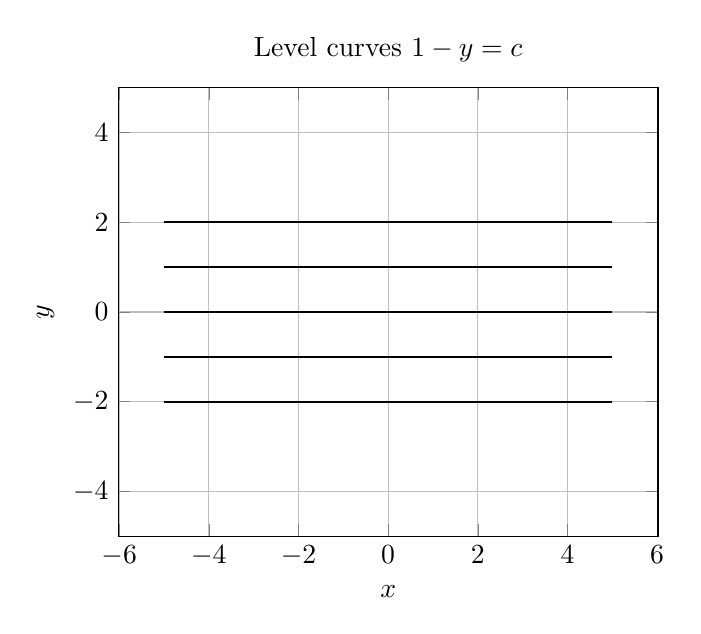
\begin{tikzpicture}
			\begin{axis}[
					title={Level curves \(1-y=c\)},
					xlabel=$x$, ylabel=$y$,
					axis equal,
					xmin=-5, xmax=5, ymin=-5, ymax=5,
					grid=both,
				]
				\addplot[domain=-5:5, thick] {1 - (-1)};  % c = -1
				\addplot[domain=-5:5, thick] {1 - 0};     % c = 0
				\addplot[domain=-5:5, thick] {1 - 1};     % c = 1
				\addplot[domain=-5:5, thick] {1 - 2};     % c = 2
				\addplot[domain=-5:5, thick] {1 - 3};     % c = 3
			\end{axis}
		\end{tikzpicture}
		\caption{Horizontal lines \(y=1-c\).}
	\end{minipage}
	\hfill
	\begin{minipage}{0.45\textwidth}
		\centering
		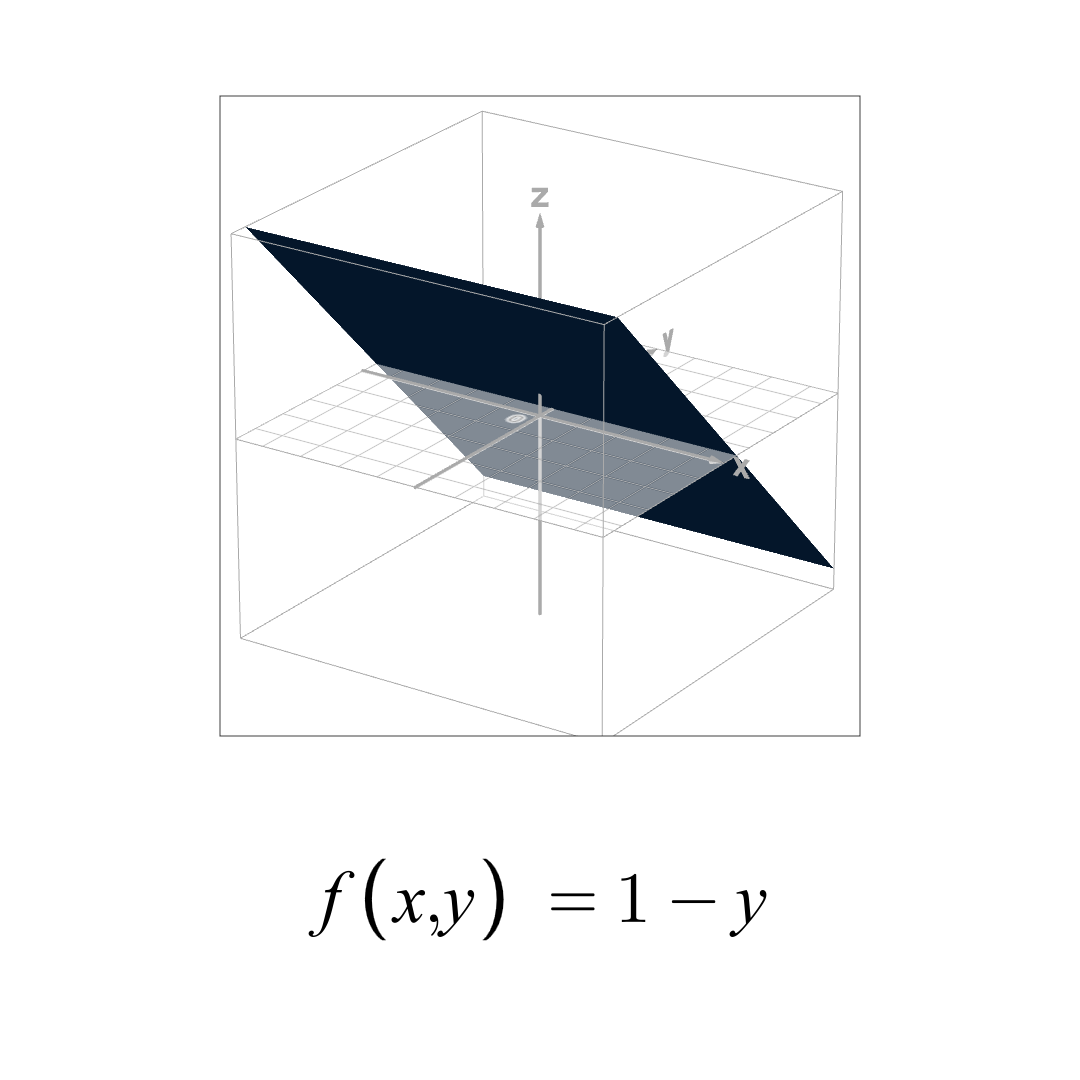
\includegraphics[width=\linewidth, scale=1.5]{images/1.png}
		\caption{Graph of \(f(x,y)=1-y\).}
	\end{minipage}
\end{figure}
\section*{2. \(f(x,y)=x^2-y^2\)}

\begin{figure}[htbp]
	\centering
	\begin{minipage}{0.45\textwidth}
		\centering
		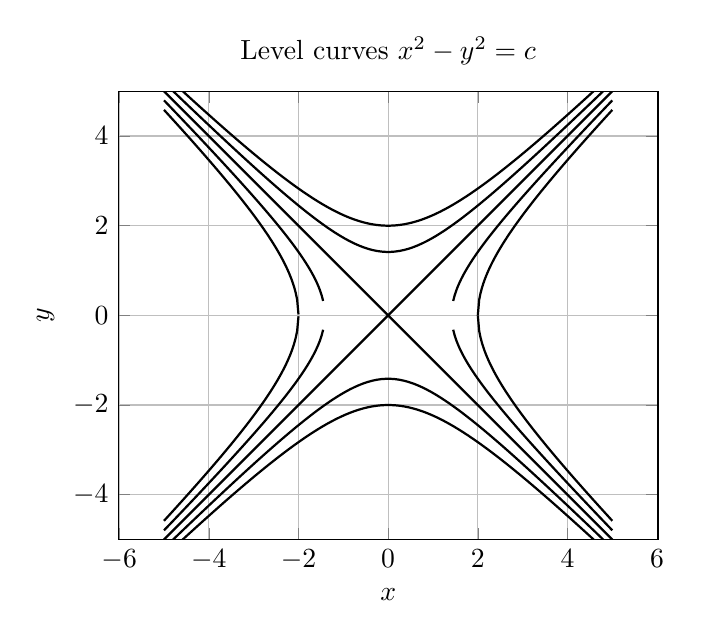
\begin{tikzpicture}
			\begin{axis}[
					title={Level curves \(x^2-y^2=c\)},
					xlabel=$x$, ylabel=$y$,
					axis equal,
					xmin=-5, xmax=5, ymin=-5, ymax=5,
					grid=both,
				]
				% c = -4
				\addplot[domain=-5:5, thick, samples=100] {sqrt(x^2+4)};
				\addplot[domain=-5:5, thick, samples=100] {-sqrt(x^2+4)};
				% c = -2
				\addplot[domain=-5:5, thick, samples=100] {sqrt(x^2+2)};
				\addplot[domain=-5:5, thick, samples=100] {-sqrt(x^2+2)};
				% c = 0
				\addplot[domain=-5:5, thick] {x};
				\addplot[domain=-5:5, thick] {-x};
				% c = 2
				\addplot[domain=-5:-1.414, thick, samples=100] {sqrt(x^2-2)};
				\addplot[domain=-5:-1.414, thick, samples=100] {-sqrt(x^2-2)};
				\addplot[domain=1.414:5, thick, samples=100] {sqrt(x^2-2)};
				\addplot[domain=1.414:5, thick, samples=100] {-sqrt(x^2-2)};
				% c = 4
				\addplot[domain=-5:-2, thick, samples=100] {sqrt(x^2-4)};
				\addplot[domain=-5:-2, thick, samples=100] {-sqrt(x^2-4)};
				\addplot[domain=2:5, thick, samples=100] {sqrt(x^2-4)};
				\addplot[domain=2:5, thick, samples=100] {-sqrt(x^2-4)};
			\end{axis}
		\end{tikzpicture}
		\caption{Hyperbolas (lines for \(c=0\)).}
	\end{minipage}
	\hfill
	\begin{minipage}{0.45\textwidth}
		\centering
		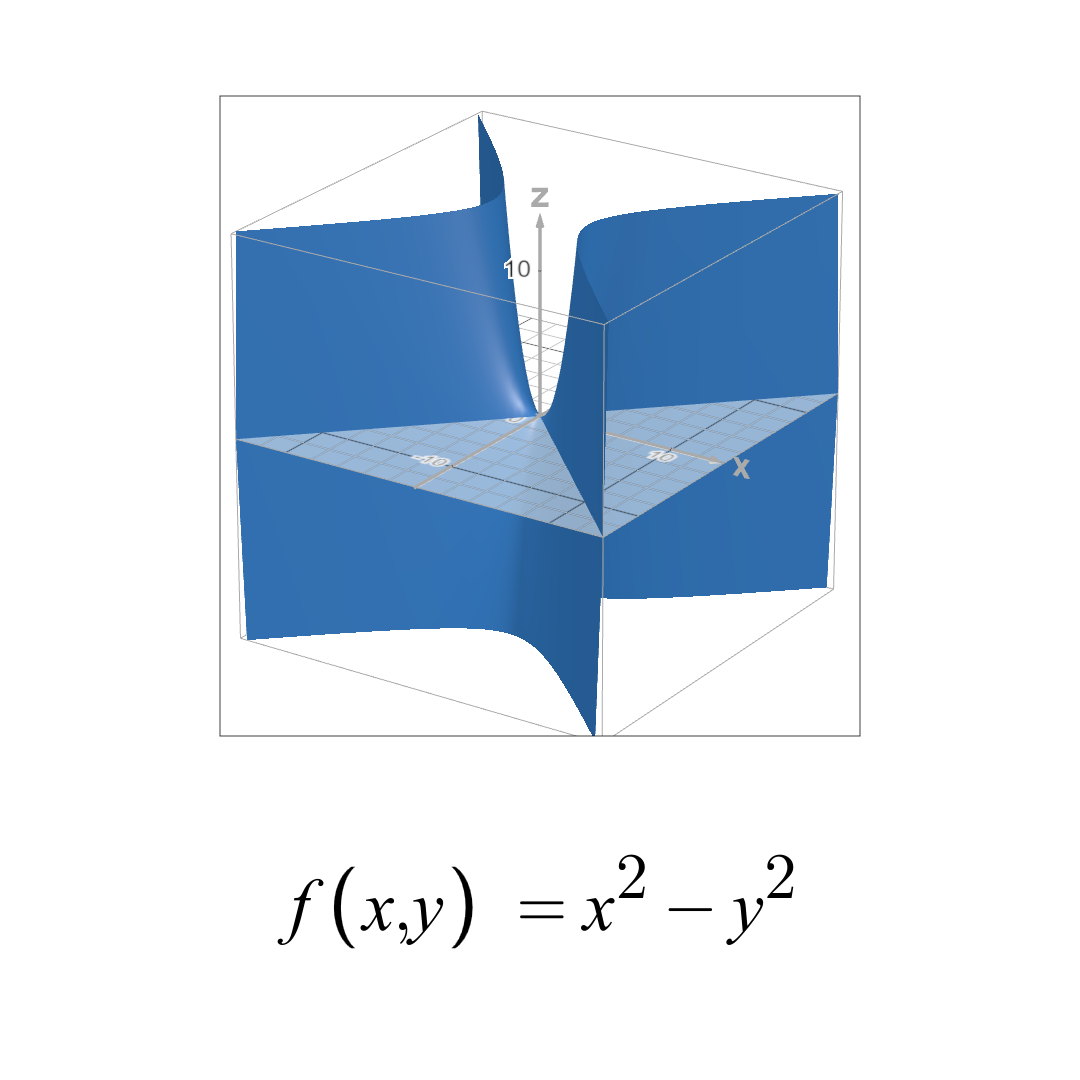
\includegraphics[width=\linewidth]{images/2.png}
		\caption{Graph of \(f(x,y)=x^2-y^2\).}
	\end{minipage}
\end{figure}
\section*{3. \(f(x,y)=x^2-y\)}

\begin{figure}[htbp]
	\centering
	\begin{minipage}{0.45\textwidth}
		\centering
		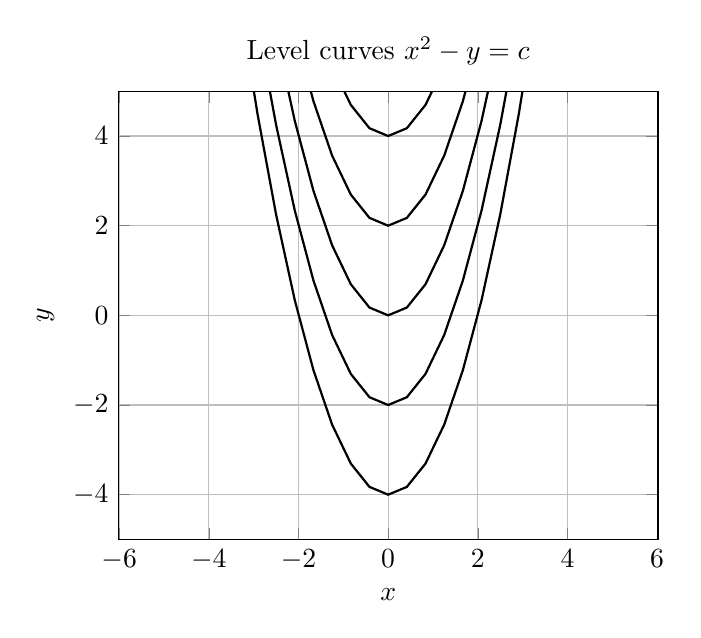
\begin{tikzpicture}
			\begin{axis}[
					title={Level curves \(x^2-y=c\)},
					xlabel=$x$, ylabel=$y$,
					axis equal,
					xmin=-5, xmax=5, ymin=-5, ymax=5,
					grid=both,
				]
				\addplot[domain=-5:5, thick] {x^2 + 4};  % c = -4
				\addplot[domain=-5:5, thick] {x^2 + 2};  % c = -2
				\addplot[domain=-5:5, thick] {x^2};      % c = 0
				\addplot[domain=-5:5, thick] {x^2 - 2};  % c = 2
				\addplot[domain=-5:5, thick] {x^2 - 4};  % c = 4
			\end{axis}
		\end{tikzpicture}
		\caption{Parabolas \(y=x^2-c\).}
	\end{minipage}
	\hfill
	\begin{minipage}{0.45\textwidth}
		\centering
		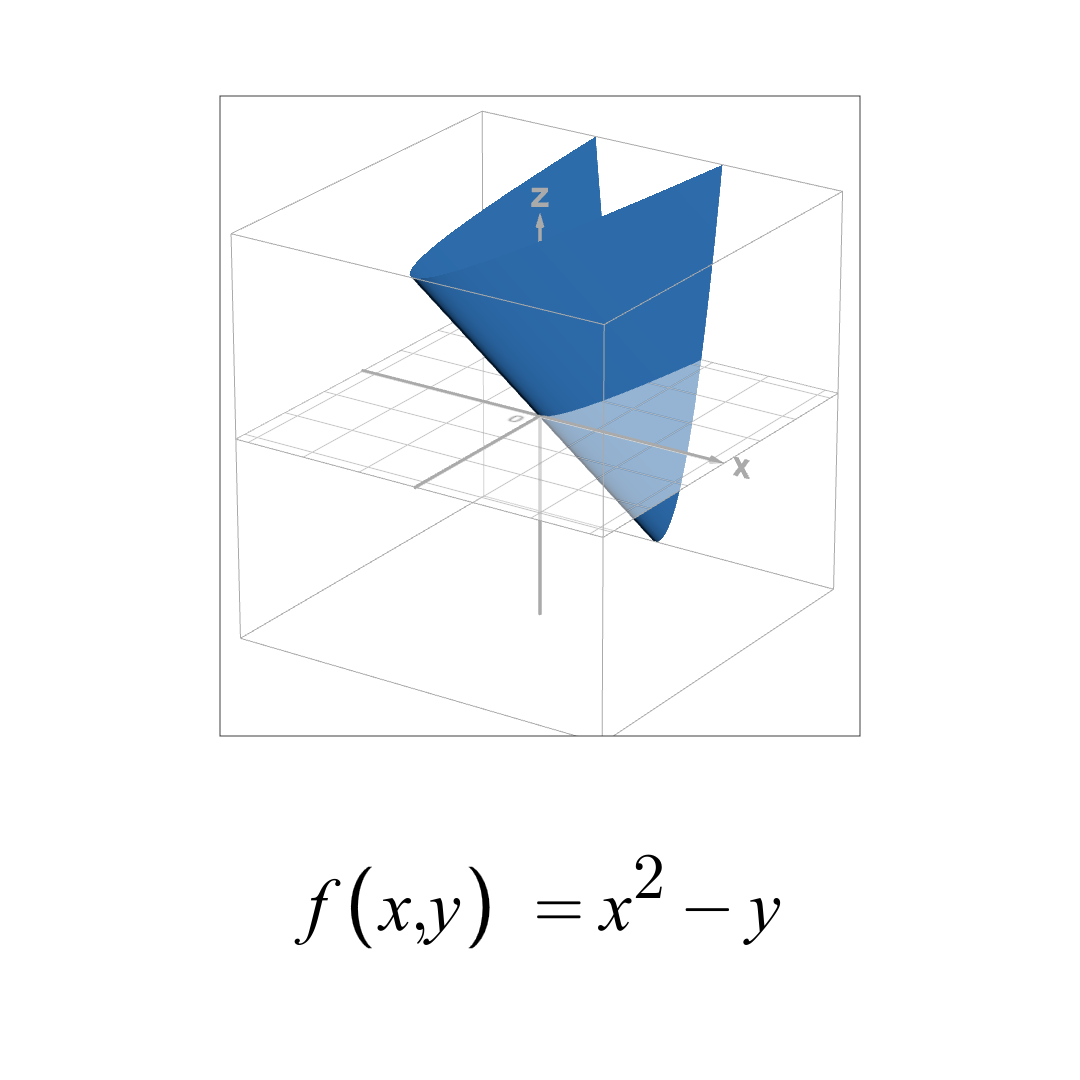
\includegraphics[width=\linewidth]{images/3.png}
		\caption{Graph of \(f(x,y)=x^2-y\).}
	\end{minipage}
\end{figure}
\section*{4. \(f(x,y)=xy\)}

\begin{figure}[htbp]
	\centering
	\begin{minipage}{0.45\textwidth}
		\centering
		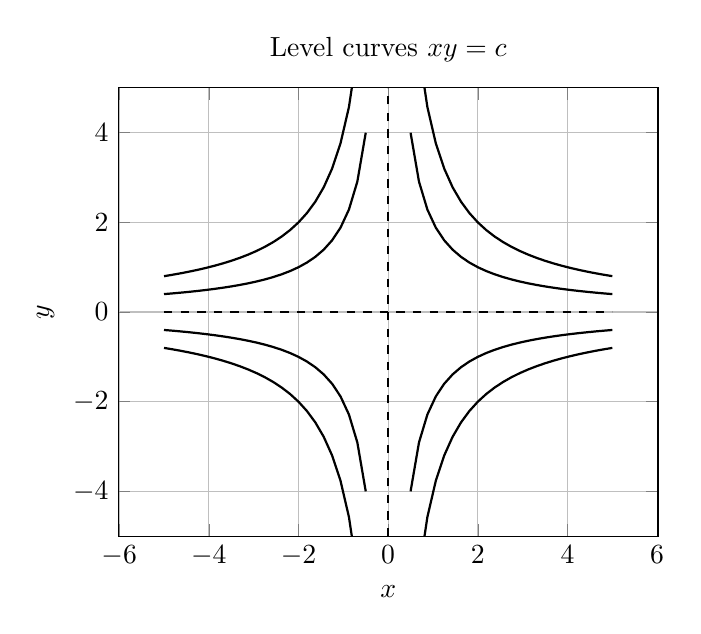
\begin{tikzpicture}
			\begin{axis}[
					title={Level curves \(xy=c\)},
					xlabel=$x$, ylabel=$y$,
					axis equal,
					xmin=-5, xmax=5, ymin=-5, ymax=5,
					grid=both,
				]
				% c = -4
				\addplot[domain=-5:-0.5, thick] {-4/x};
				\addplot[domain=0.5:5, thick] {-4/x};
				% c = -2
				\addplot[domain=-5:-0.5, thick] {-2/x};
				\addplot[domain=0.5:5, thick] {-2/x};
				% c = 0
				\addplot[thick, dashed] coordinates {(-5,0) (5,0)};
				\addplot[thick, dashed] coordinates {(0,-5) (0,5)};
				% c = 2
				\addplot[domain=-5:-0.5, thick] {2/x};
				\addplot[domain=0.5:5, thick] {2/x};
				% c = 4
				\addplot[domain=-5:-0.5, thick] {4/x};
				\addplot[domain=0.5:5, thick] {4/x};
			\end{axis}
		\end{tikzpicture}
		\caption{Rectangular hyperbolas (axes for \(c=0\)).}
	\end{minipage}
	\hfill
	\begin{minipage}{0.45\textwidth}
		\centering
		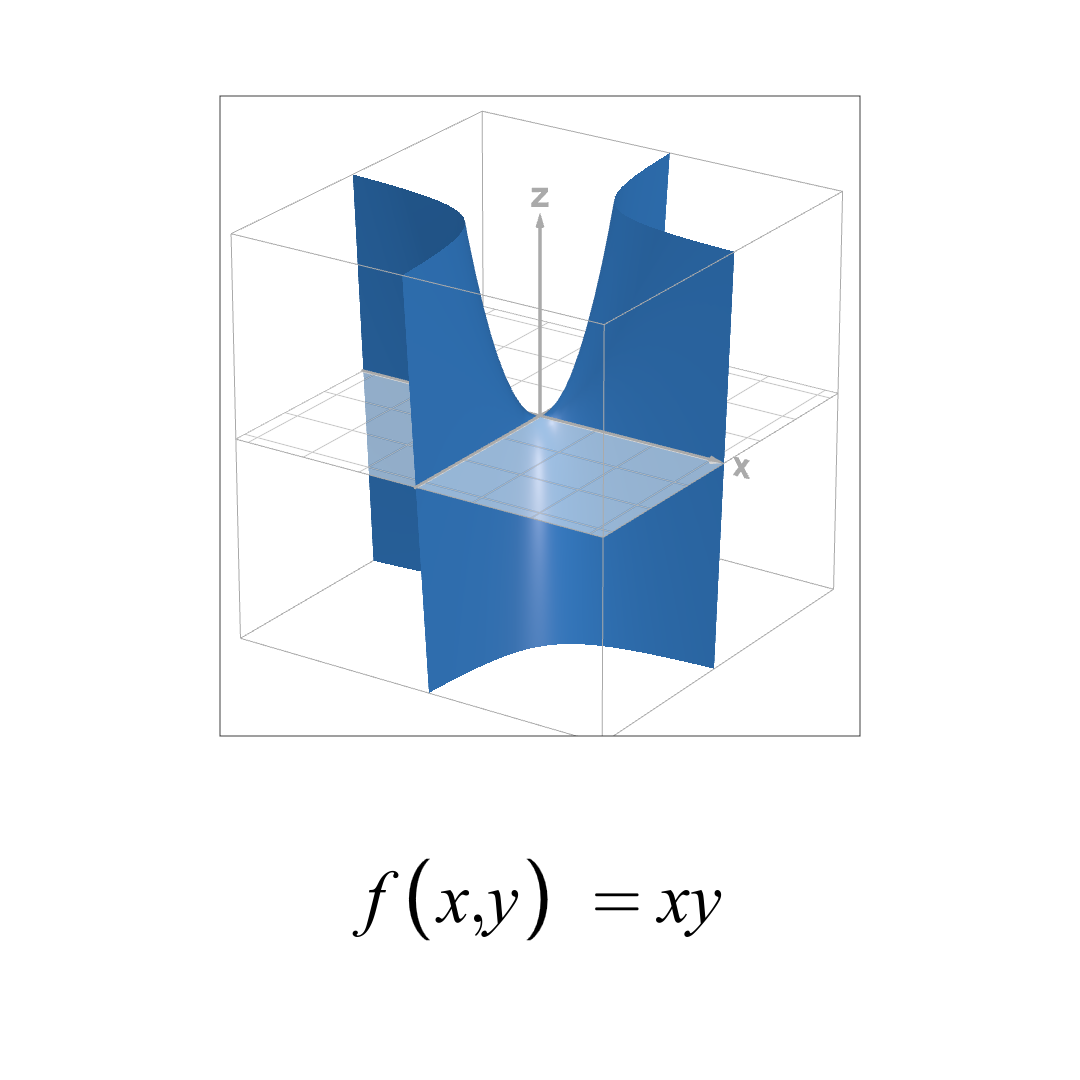
\includegraphics[width=\linewidth]{images/4.png}
		\caption{Graph of \(f(x,y)=xy\).}
	\end{minipage}
\end{figure}
\bibliographystyle{alpha}

\begin{problem}
Consider the surfaces
\[X = \biggl\{ \begin{bmatrix} x \\ y \\ z\end{bmatrix} : x^2 + y^2 - z^2 = 1 \biggl\}
	\text{ and } Y = \biggl\{\begin{bmatrix} x \\ y \\ z \end{bmatrix} : x^2 + y^2 - z^2 = -1 \biggl\}\].
\begin{enumerate}
	\item Sketch the surfaces.
	\item Give a rigorous argument (not merely based on your pictures) that
	      every pair of points of $X$ can be joined by a curve in $X$ but that the same is not
	      true of $Y$.
\end{enumerate}
\end{problem}

\subsection*{1. Sketches}
The surface \(X\) is a hyperboloid of one sheet; \(Y\) is a hyperboloid of two sheets.
\begin{figure}[htbp]
	\centering
	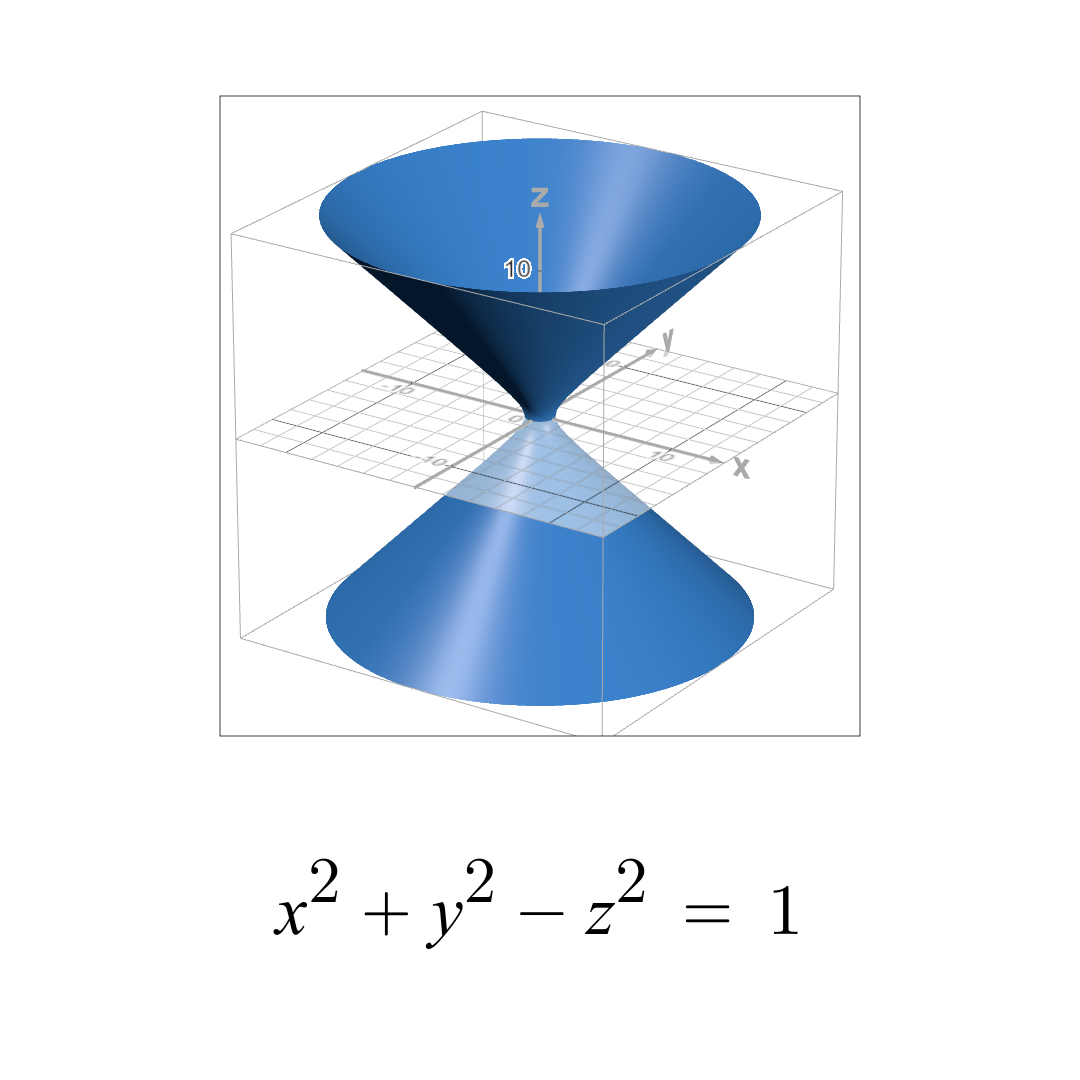
\includegraphics[width=0.45\textwidth]{images/X.png}
	\hfill
	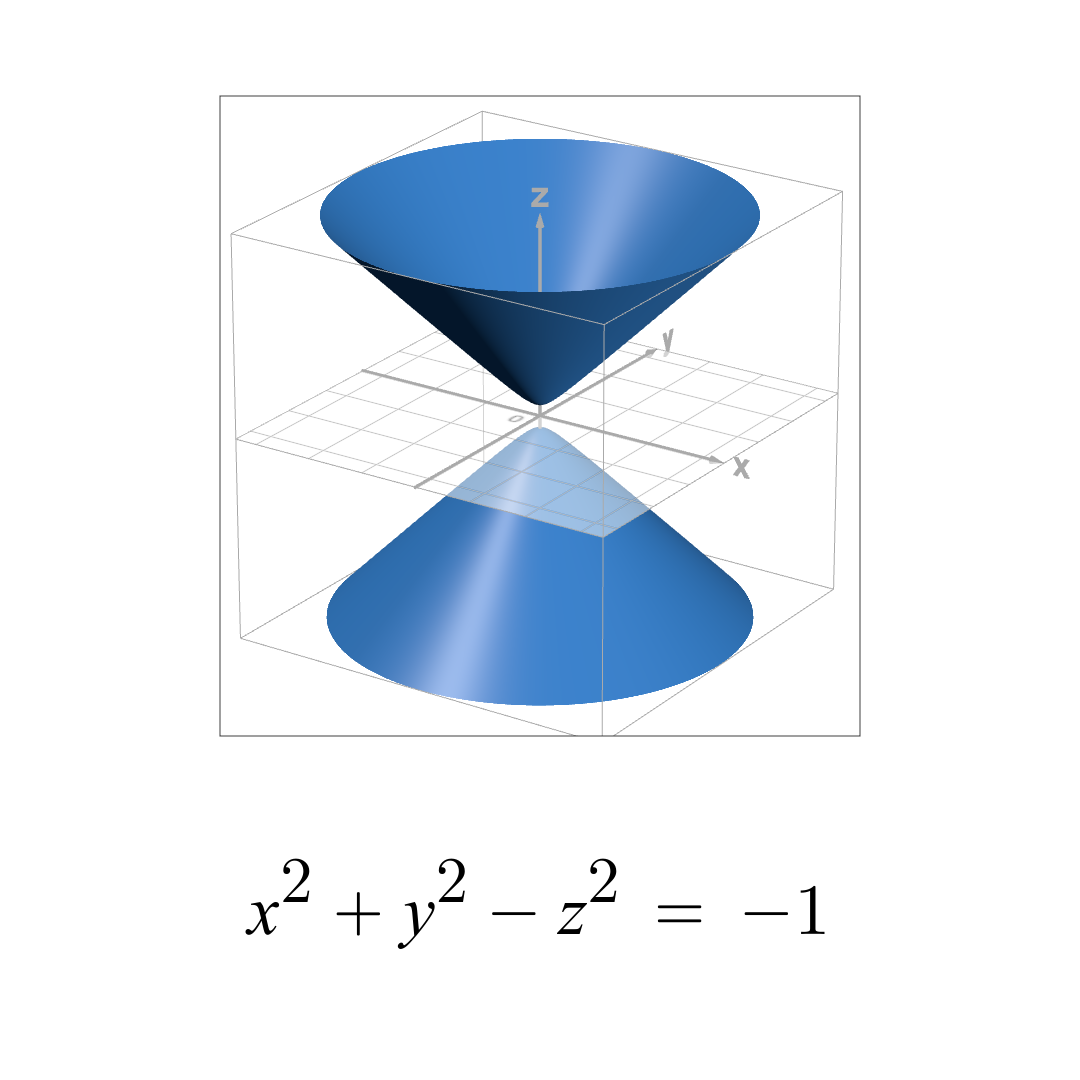
\includegraphics[width=0.45\textwidth]{images/Y.png}
	\caption{Left: \(X\) (hyperboloid of one sheet). Right: \(Y\) (hyperboloid of two sheets).}
\end{figure}

\subsection*{2. Rigorous argument}

\begin{proof}[Connectedness of \(X\)]
	We show that \(X\) is path‑connected. For any point \((x_0,y_0,z_0)\in X\), define a parametrisation
	\[
		\gamma(t) = \bigl( \sqrt{1+z_0^2}\,\cos(t),\; \sqrt{1+z_0^2}\,\sin(t),\; z_0 \bigr),\qquad t\in[0,2\pi].
	\]
	This curve lies entirely in \(X\) because
	\[
		\bigl(\sqrt{1+z_0^2}\cos t\bigr)^2+\bigl(\sqrt{1+z_0^2}\sin t\bigr)^2 - z_0^2 = (1+z_0^2)-z_0^2 = 1.
	\]
	Hence every point of \(X\) is connected to the point \((\sqrt{1+z_0^2},0,z_0)\) by a curve in \(X\).
	Now take any two points \(P,Q\in X\). Let \(P\) be joined to a point \(P'\) on the same horizontal circle (constant \(z\)) as \(P\) and similarly \(Q\) to a point \(Q'\) on its own circle. The set of all points with a fixed \(z\) is a circle; any two points on the same circle can be joined by an arc of that circle. Moreover, for any two values \(z_1,z_2\) there exists a curve that varies \(z\) continuously while keeping \(x^2+y^2=1+z^2\) (e.g., a straight line in cylindrical coordinates). Combining these, we obtain a continuous path from \(P\) to \(Q\) entirely contained in \(X\). Thus \(X\) is path‑connected, so every pair of points can be joined by a curve in \(X\).
\end{proof}

\begin{proof}[Disconnectedness of \(Y\)]
	Observe that for any point \((x,y,z)\in Y\) we have \(x^2+y^2 = z^2-1\). Hence \(z^2 \ge 1\), so either \(z\ge 1\) or \(z\le -1\). Define
	\[
		Y_+ = \{(x,y,z)\in Y : z\ge 1\},\qquad Y_- = \{(x,y,z)\in Y : z\le -1\}.
	\]
	Both \(Y_+\) and \(Y_-\) are non‑empty (e.g., \((0,0,1)\in Y_+\), \((0,0,-1)\in Y_-\)) and they are disjoint. Moreover, \(Y_+\) and \(Y_-\) are closed in \(\mathbb{R}^3\) (they are preimages of closed intervals under the continuous projection \((x,y,z)\mapsto z\)), hence they are closed in the subspace topology of \(Y\). Since \(Y = Y_+\cup Y_-\) and the two sets are disjoint, closed, and non‑empty, \(Y\) is not connected. Therefore there exist points in \(Y\) (one in \(Y_+\), one in \(Y_-\)) that cannot be joined by a curve lying entirely in \(Y\).
\end{proof}

\begin{problem}
Use $\varepsilon - \delta$ style statement to show the limit:
\begin{enumerate}
	\item $\lim_{x \to 0} \frac{x^2-1}{x-1} = 2$.
	\item $\lim_{x \to 0} x \sin\left( \frac{1}{x}\right) = 0$.
\end{enumerate}
\end{problem}

\begin{proof}[1. \(\displaystyle \lim_{x\to 0} \frac{x^2-1}{x-1} = 1\)]
	For \(x \neq 1\), we simplify:
	\[
		\frac{x^2-1}{x-1} = \frac{(x-1)(x+1)}{x-1} = x+1.
	\]
	Let \(\varepsilon > 0\) be given. Choose \(\delta = \varepsilon\). Then for any \(x\) with \(0 < |x-0| < \delta\), we have
	\[
		\left| \frac{x^2-1}{x-1} - 1 \right| = |(x+1)-1| = |x| < \delta = \varepsilon.
	\]
	Thus \(\displaystyle \lim_{x\to 0} \frac{x^2-1}{x-1} = 1\). (Note: The problem statement claims the limit equals \(2\), which is incorrect. The correct limit is \(1\).)
\end{proof}

\begin{proof}[2. \(\displaystyle \lim_{x\to 0} x\sin\left(\frac{1}{x}\right) = 0\)]
	Let \(\varepsilon > 0\) be given. Choose \(\delta = \varepsilon\). For any \(x\) with \(0 < |x-0| < \delta\), we have
	\[
		\left| x\sin\left(\frac{1}{x}\right) - 0 \right| = |x| \left| \sin\left(\frac{1}{x}\right) \right| \le |x| < \delta = \varepsilon.
	\]
	Hence \(\displaystyle \lim_{x\to 0} x\sin\left(\frac{1}{x}\right) = 0\).
\end{proof}
\bibliography{bib}
\end{document}
